\chapter{Przygotowanie odpowiedzi skokowych do regulatora DMC oraz ich aproksymacja}

\section{Odpowiedzi skokowe}

Jako parametry regulatora DMC zosta�y wybrane odpowiedzi skokowe dla dw�ch oddzielnych zmian warto�ci sterowania $G1$ z \num{18} na \num{38} i $G2$ \num{23} na \num{43} z punktu pracy.

\begin{figure}
	\centering
	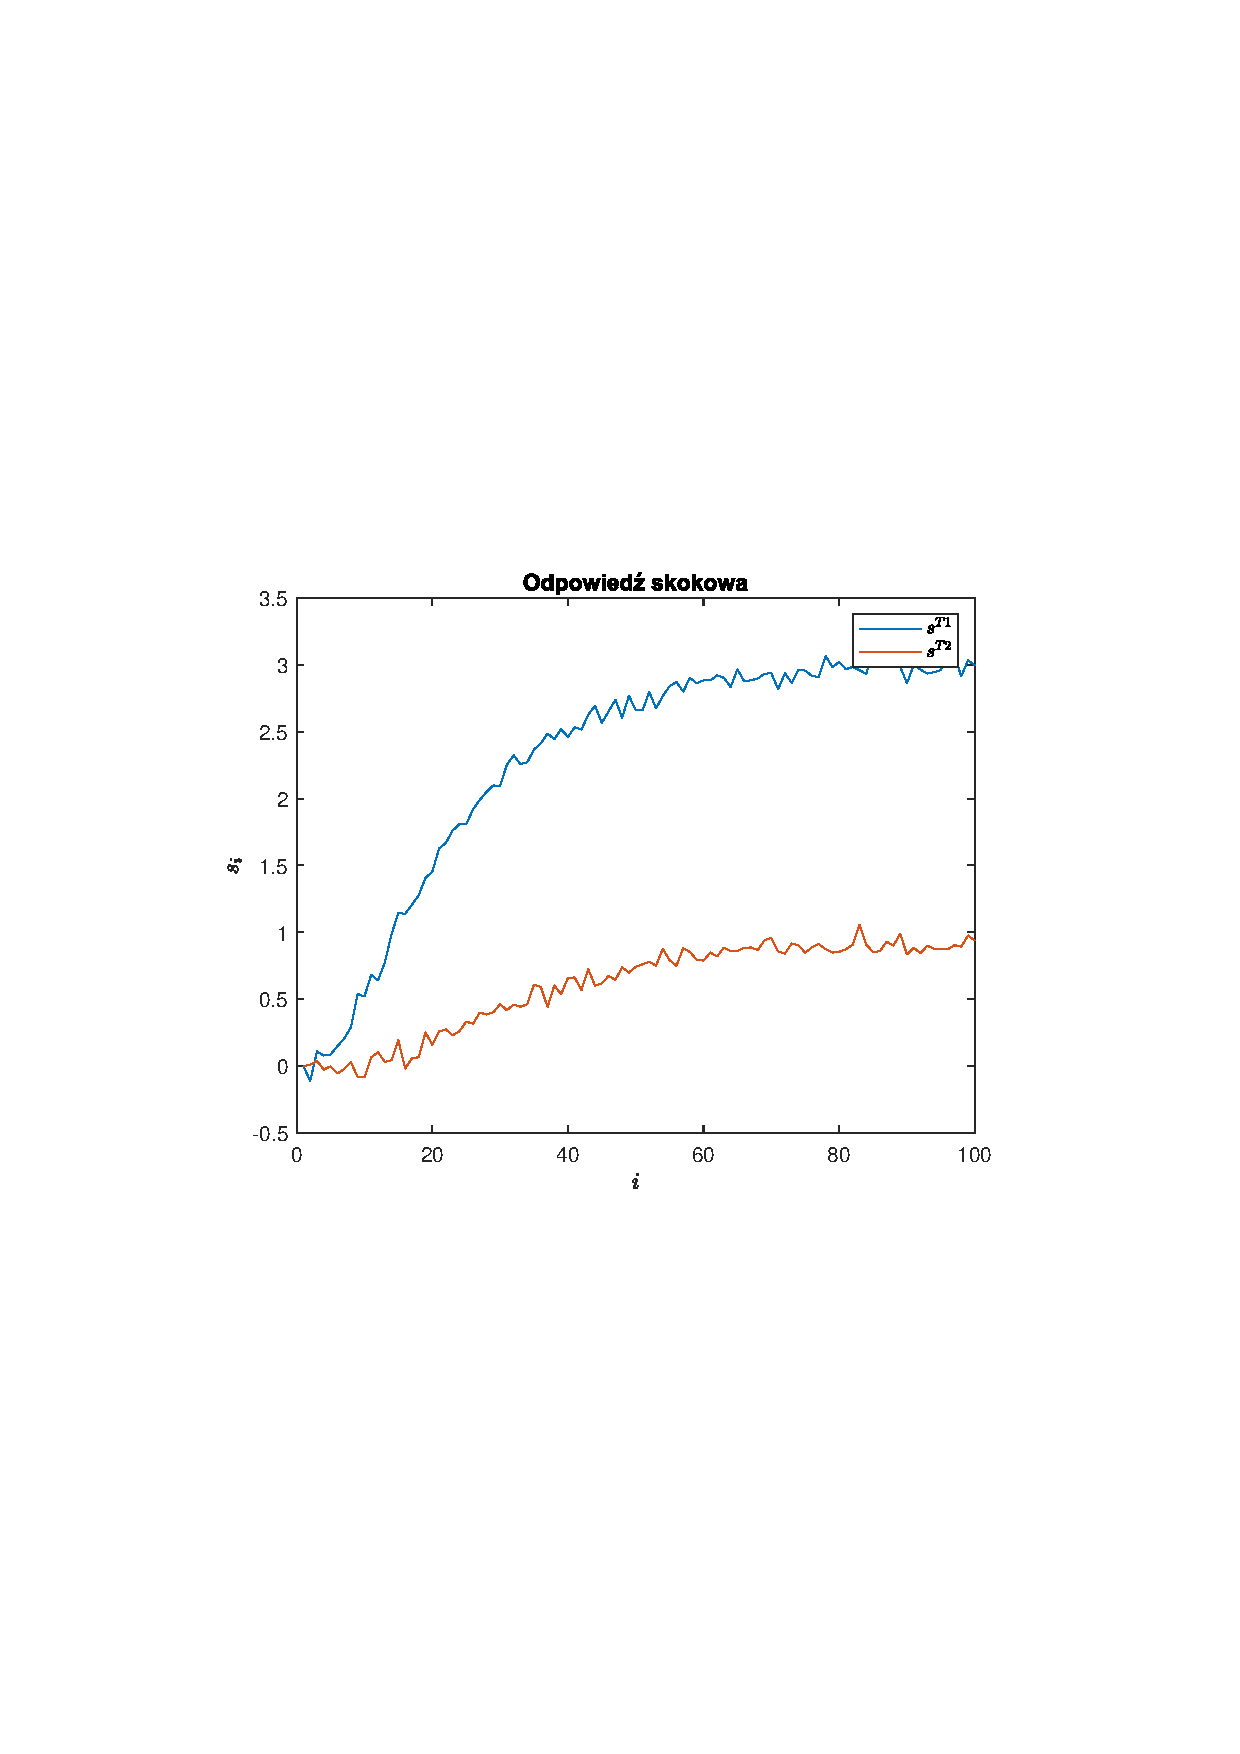
\includegraphics[scale=0.85, trim={2cm 8.5cm 2cm 8.5cm}]{rysunki/odp_skok_g1}
	\caption{Odpowied� skokowa dla zmiany sygna�u sterowania $G1$ z $\num{18}$ na $\num{38}$  z punktu pracy}
	\label{odp_skok_g1}
\end{figure}

\begin{figure}
	\centering
	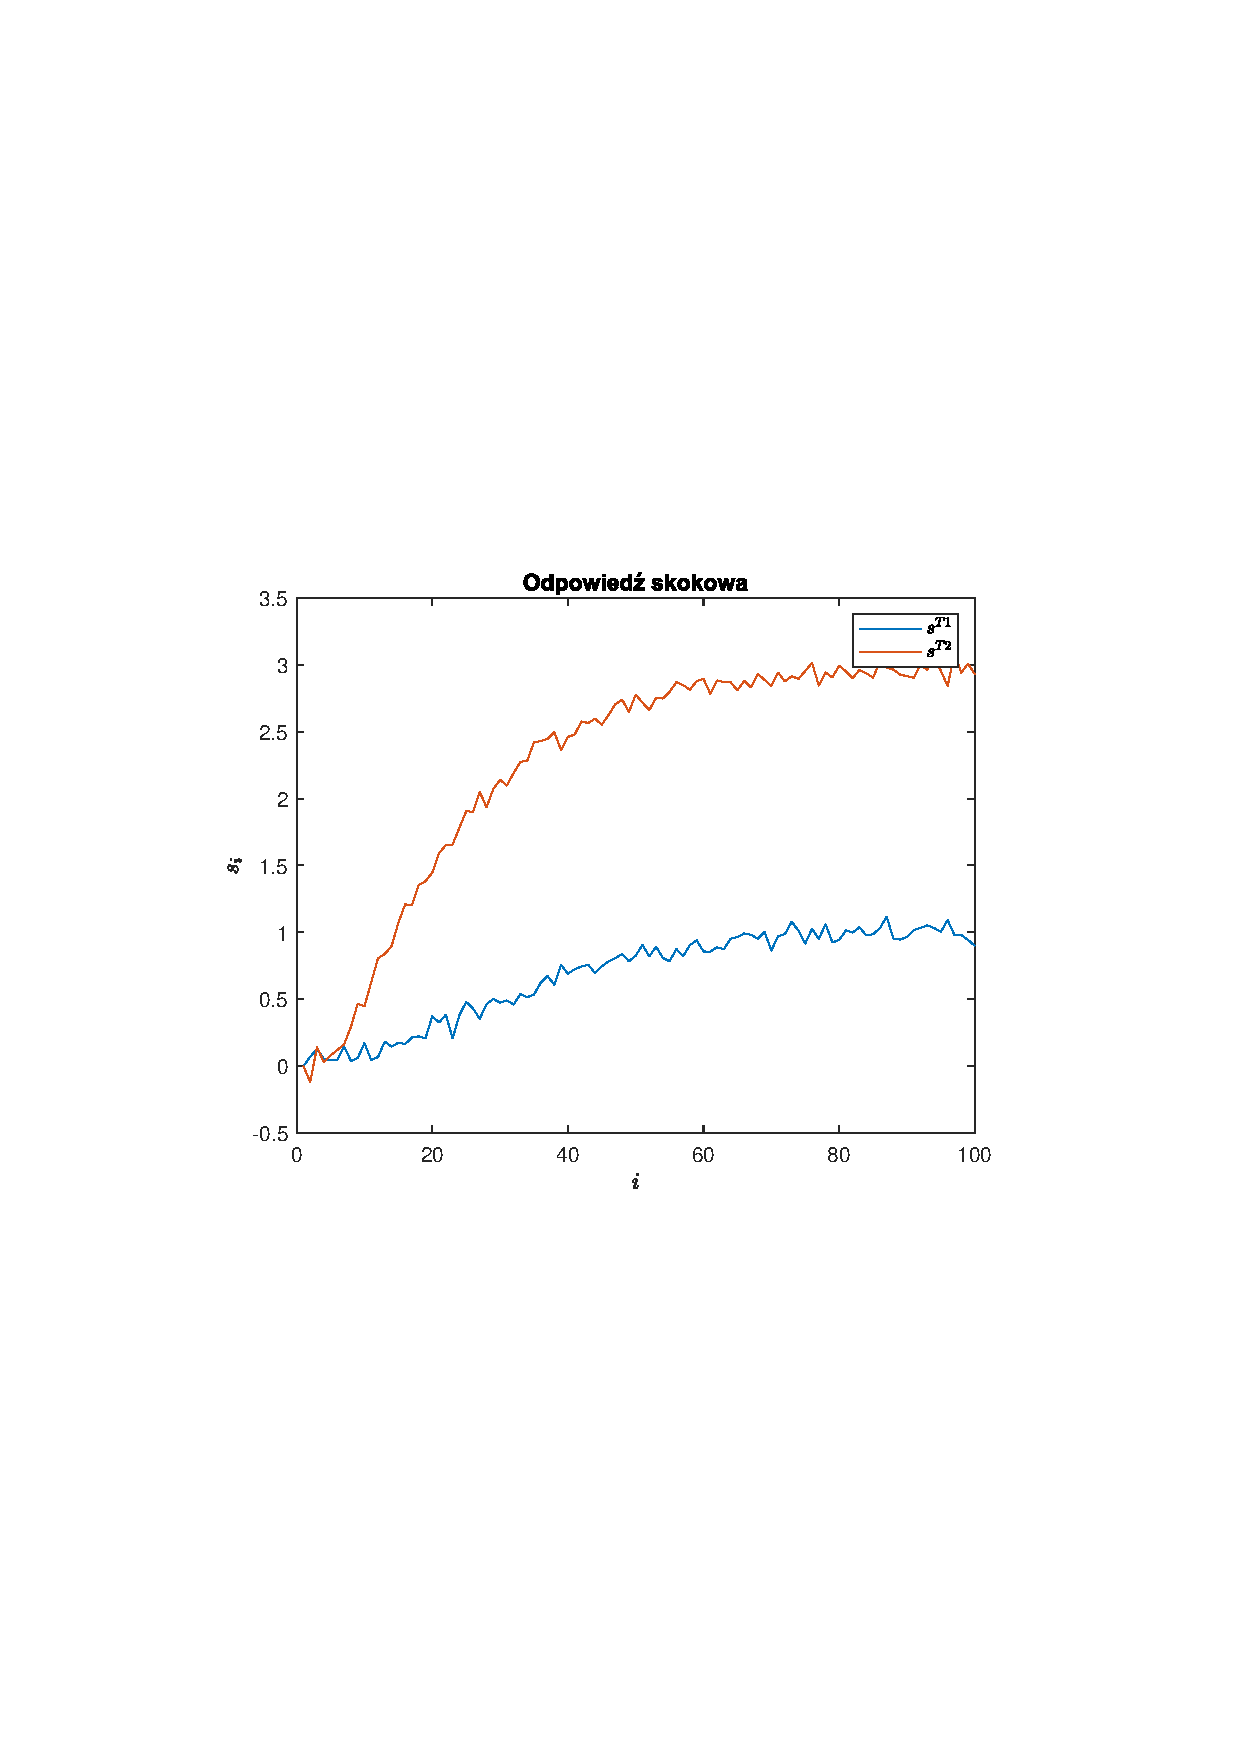
\includegraphics[scale=0.85, trim={2cm 8.5cm 2cm 8.5cm}]{rysunki/odp_skok_g2}
	\caption{Odpowied� skokowa dla zmiany sygna�u sterowania $G2$ z $\num{23}$ na $\num{43}$  z punktu pracy}
	\label{odp_skok_g2}
\end{figure}

\subsection{Implementacja}

Do zrealizowania zadania zosta�y u�yte skrypty \verb+zad2.m+ oraz \verb+odp_skok.m+.

\section{Aproksymacja odpowiedzi skokowych}

Do zaaproksymowania odpowiedzi skokowych zosta� u�yty cz�on inercyjny drugiego rz�du z op�nieniem o nast�puj�cej postaci:

\begin{equation}
	G(s) = \frac{K}{(sT_1+1)(sT_2+1)}e^{-T_\textrm{d}s}
\end{equation}

czyli po zastosowaniu transformaty $Z$

\begin{equation}
G(z) = \frac{b_1z^{-1}+b_2z^{-2}}{1+a_1z^{-1}+a_2z^{-2}}z^{-T_\mathrm{d}}
\end{equation}

gdzie

\begin{align*} 
a_1 =& -\alpha_1-\alpha_2 \\ 
a_2 =& \alpha_1\alpha_2 \\
\alpha_1 =& e^{-\frac{1}{T_1}} \\
\alpha_2 =& e^{-\frac{1}{T_2}} \\
b_1 =& \frac{K}{T_1-T_2}[T_1(1-\alpha_1)-T_2(1-\alpha_2)] \\ 
b_2 =& \frac{K}{T_1-T_2}[\alpha_1T_2(1-\alpha_2)-\alpha_2T_1(1-\alpha_1)]
\end{align*}

co przek�ada si� na r�wnianie r�nicowe o postaci:

\begin{equation}
	y(k) = b_1u(k-T_\mathrm{D}-1) + b_2u(k-T_\mathrm{D}-2) - a_1y(k-1) - a_2y(k-2)
\end{equation}

Bior�c pod uwag� ograniczenie co do dziedziny parametru $T_\mathrm{d}$ (liczba ca�kowita) zdecydowali�my si� u�y� algorytmu genetycznego w celu dobrania parametr�w $T_1$, $T_2$, $K$, $T_\mathrm{d}$ cz�onu aproksymuj�cego odpowied� skokow�. Wska�nikiem ilo�ciowym wykorzystanym do optymalizacji zosta�a funkcja sumy kwadrat�w r�nicy. 

\begin{equation}
E = \sum^{\mathrm{D}}_{i=1}(s_i-\widehat{s}_i)^2
\end{equation}

,gdzie $\widehat{s}$ jest aproksymacj�.

Do obliczenia optymalnych parametr�w u�yli�my funkcji \texttt{ga} (Algorytm Genetyczny) z pakietu \texttt{Global Optimization Toolbox}.

\begin{figure}
	\centering
	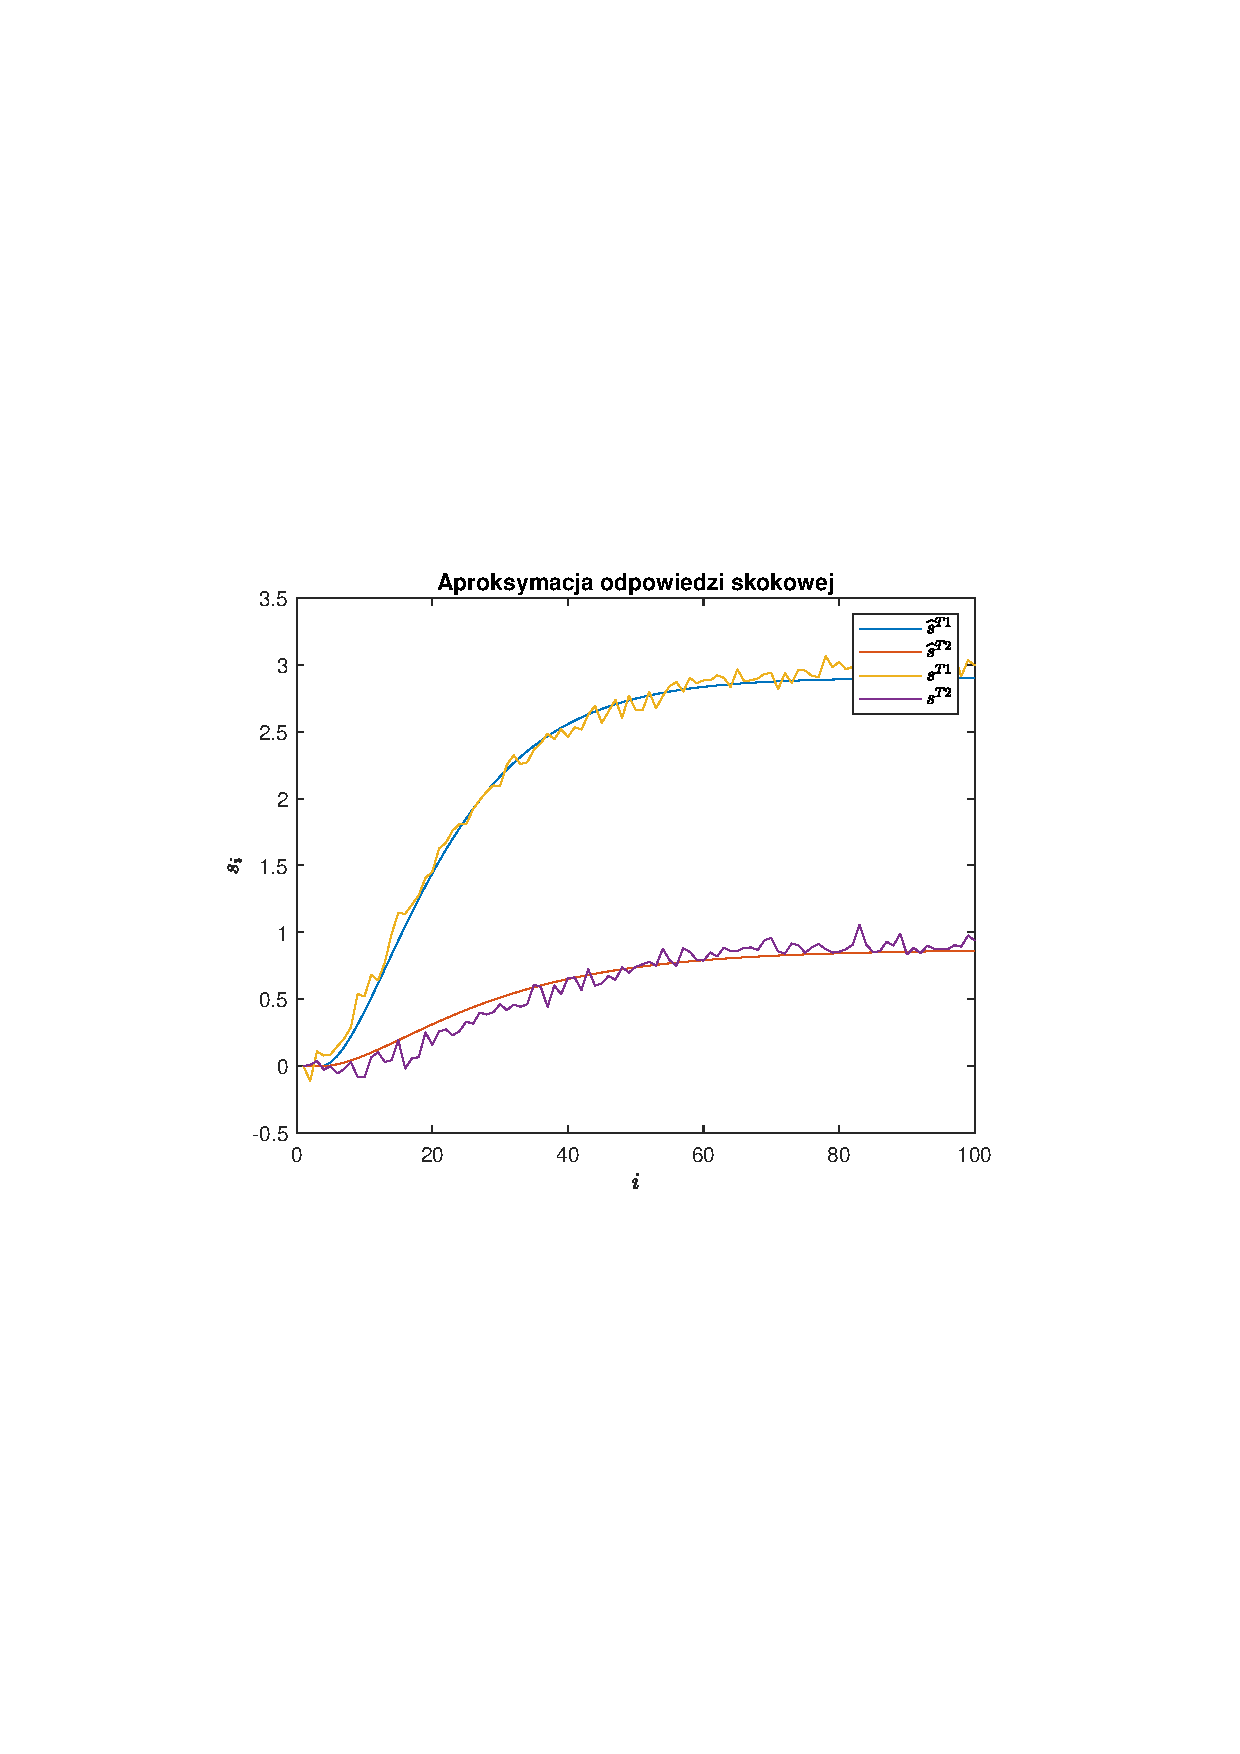
\includegraphics[scale=0.85, trim={2cm 8.5cm 2cm 8.5cm}]{rysunki/odp_skok_g1_aproksym}
	\caption{Aproksymacja odpowiedzi skokowej dla zmiany sygna�u sterowania $G1$ z $\num{18}$ na $\num{38}$  z punktu pracy}
	\label{odp_skok_g1_aproksym}
\end{figure}

\begin{figure}
	\centering
	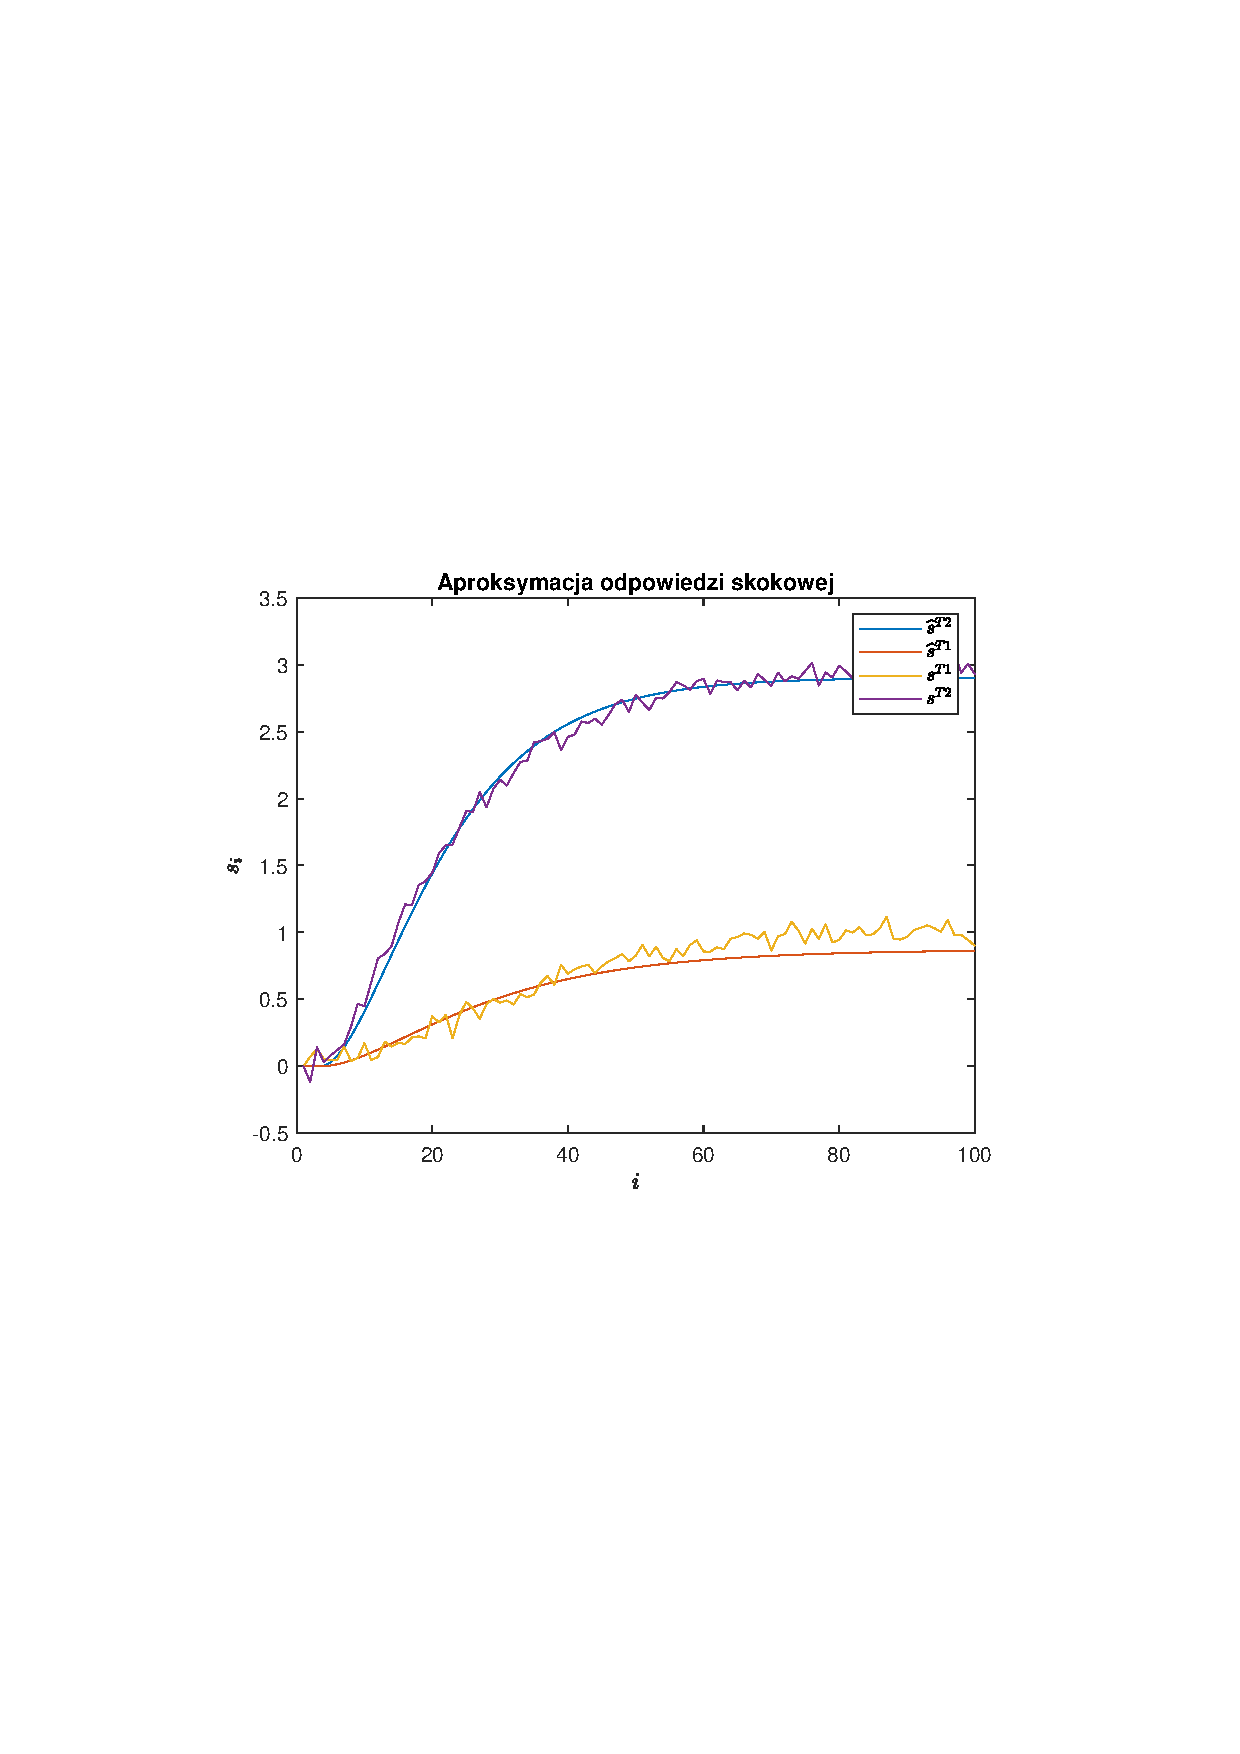
\includegraphics[scale=0.85, trim={2cm 8.5cm 2cm 8.5cm}]{rysunki/odp_skok_g2_aproksym}
	\caption{Aproksymacja odpowiedzi skokowej dla zmiany sygna�u sterowania $G2$ z $\num{23}$ na $\num{43}$  z punktu pracy}
	\label{odp_skok_g2_aproksym}
\end{figure}

\subsection{Implementacja}

Do zrealizowania zadania zosta�y u�yte skrypty \verb+odpSkokAproksymowane.m+ (g��wny skrypt wyliczaj�cy odpowiedzi apkroksymowane oraz rysuj�cy wykresy) oraz \verb+coeffOptim.m+ (funkcja celu do zminimalizowania).
